O colesterol total de uma pessoa � obtido pela soma da taxa do seu "colesterol bom" com a taxa do seu "colesterol ruim". Os exames peri�dicos, realizados em um paciente adulto, apresentaram taxa normal de "colesterol bom", por�m, taxa do "colesterol ruim" (tamb�m chamado LDL) de 280 mg/dl. 
O quadro apresenta uma classifica��o de acordo com as taxas de LDL em adultos. 

\begin{figure}[h]
\centering
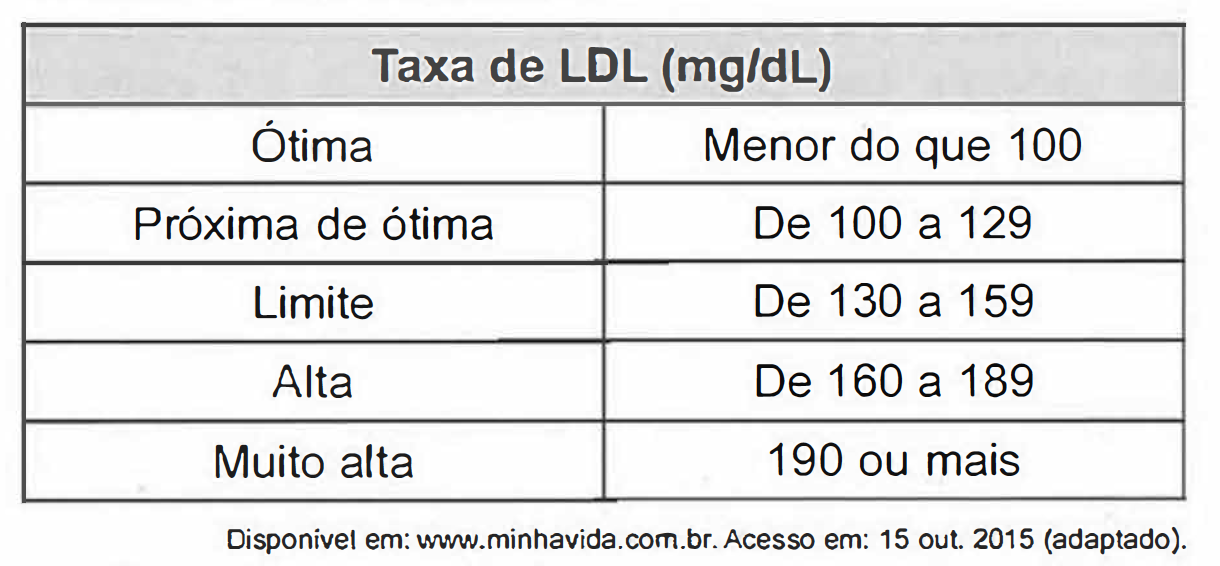
\includegraphics[width=8cm]{../figuras/q163-2018.png}
\end{figure}

O paciente, seguindo as recomenda��es m�dicas sobre estilo de vida e alimenta��o, realizou o exame logo ap�s o primeiro m�s, e a taxa de LDL reduziu 25\%. No m�s seguinte, realizou novo exame e constatou uma redu��o de mais 20\% na taxa de LDL. 
De acordo com o resultado do segundo exame, a classifica��o da taxa de LDL do paciente � 

\begin{enumerate}
\item[a)]�tima
\item[b)]pr�xima de �tima.
\item[c)]limite.
\item[d)]alta.
\item[e)]muito alta
\end{enumerate}